%
%Не забыть:
%--------------------------------------
%Вставить колонтитулы, поменять название на титульнике



%--------------------------------------

\documentclass[a4paper, 12pt]{article} 

%--------------------------------------
%Russian-specific packages
%--------------------------------------
%\usepackage[warn]{mathtext}
\usepackage[T2A]{fontenc}
\usepackage[utf8]{inputenc}
\usepackage[english,russian]{babel}
\usepackage[intlimits]{amsmath}
\usepackage{esint}
%--------------------------------------
%Hyphenation rules
%--------------------------------------
\usepackage{hyphenat}
\hyphenation{ма-те-ма-ти-ка вос-ста-нав-ли-вать}
%--------------------------------------
%Packages
%--------------------------------------
\usepackage{amsmath}
\usepackage{amssymb}
\usepackage{amsfonts}
\usepackage{amsthm}
\usepackage{latexsym}
\usepackage{mathtools}
\usepackage{etoolbox}%Булевые операторы
\usepackage{enumerate}% Больше опций для enumerate
\usepackage{extsizes}%Выставление произвольного шрифта в \documentclass
\usepackage{geometry}%Разметка листа
\usepackage{indentfirst}
\usepackage{wrapfig}%Создание обтекаемых текстом объектов
\usepackage{fancyhdr}%Создание колонтитулов
\usepackage{setspace}%Настройка интерлиньяжа
\usepackage{lastpage}%Вывод номера последней страницы в документе, \lastpage
\usepackage{soul}%Изменение параметров начертания
\usepackage{hyperref}%Две строчки с настройкой гиперссылок внутри получаеммого
\usepackage[usenames,dvipsnames,svgnames,table,rgb]{xcolor}% pdf-документа
\usepackage{multicol}%Позволяет писать текст в несколько колонок
\usepackage{cite}%Работа с библиографией
\usepackage{subfigure}% Человеческая вставка нескольких картинок
\usepackage{tikz}%Рисование рисунков
\usepackage{float}% Возможность ставить H в положениях картинки
% Для картинок Моти
\usepackage{misccorr}
\usepackage{lscape}
\usepackage{cmap}

% Для Х И М И И

\usepackage{mhchem}



\usepackage{graphicx,xcolor}
\graphicspath{{Pictures/}}
\DeclareGraphicsExtensions{.pdf,.png,.jpg}

%----------------------------------------
%Список окружений
%----------------------------------------
\newenvironment {theor}[2]
{\smallskip \par \textbf{#1.} \textit{#2}  \par $\blacktriangleleft$}
{\flushright{$\blacktriangleright$} \medskip \par} %лемма/теорема с доказательством
\newenvironment {proofn}
{\par $\blacktriangleleft$}
{$\blacktriangleright$ \par} %доказательство
%----------------------------------------
%Список команд
%----------------------------------------
\newcommand{\grad}
{\mathop{\mathrm{grad}}\nolimits\,} %градиент

\newcommand{\diver}
{\mathop{\mathrm{div}}\nolimits\,} %дивергенция

\newcommand{\rot}
{\ensuremath{\mathrm{rot}}\,}

\newcommand{\Def}[1]
{\underline{\textbf{#1}}} %определение

\newcommand{\RN}[1]
{\MakeUppercase{\romannumeral #1}} %римские цифры

\newcommand {\theornp}[2]
{\textbf{#1.} \textit{ #2} \par} %Написание леммы/теоремы без доказательства

\newcommand{\qrq}
{\ensuremath{\quad \Rightarrow \quad}} %Человеческий знак следствия

\newcommand{\qlrq}
{\ensuremath{\quad \Leftrightarrow \quad}} %Человеческий знак равносильности

\renewcommand{\phi}{\varphi} %Нормальный знак фи

\newcommand{\me}
{\ensuremath{\mathbb{E}}}

\newcommand{\md}
{\ensuremath{\mathbb{D}}}



%\renewcommand{\vec}{\overline}




%----------------------------------------
%Разметка листа
%----------------------------------------
\geometry{top = 3cm}
\geometry{bottom = 2cm}
\geometry{left = 1.5cm}
\geometry{right = 1.5cm}
%----------------------------------------
%Колонтитулы
%----------------------------------------
\pagestyle{fancy}%Создание колонтитулов
\fancyhead{}
%\fancyfoot{}
%----------------------------------------
%Интерлиньяж (расстояния между строчками)
%----------------------------------------
%\onehalfspacing -- интерлиньяж 1.5
%\doublespacing -- интерлиньяж 2
%----------------------------------------
%Настройка гиперссылок
%----------------------------------------
\hypersetup{				% Гиперссылки
	unicode=true,           % русские буквы в раздела PDF
	pdftitle={Заголовок},   % Заголовок
	pdfauthor={Автор},      % Автор
	pdfsubject={Тема},      % Тема
	pdfcreator={Создатель}, % Создатель
	pdfproducer={Производитель}, % Производитель
	pdfkeywords={keyword1} {key2} {key3}, % Ключевые слова
	colorlinks=true,       	% false: ссылки в рамках; true: цветные ссылки
	linkcolor=blue,          % внутренние ссылки
	citecolor=blue,        % на библиографию
	filecolor=magenta,      % на файлы
	urlcolor=cyan           % на URL
}
%----------------------------------------
%Работа с библиографией (как бич)
%----------------------------------------
\renewcommand{\refname}{Список литературы}%Изменение названия списка литературы для article
%\renewcommand{\bibname}{Список литературы}%Изменение названия списка литературы для book и report
%----------------------------------------
\begin{document}
	\begin{titlepage}
		\begin{center}
			$$$$
			$$$$
			$$$$
			$$$$
			{\Large{НАЦИОНАЛЬНЫЙ ИССЛЕДОВАТЕЛЬСКИЙ УНИВЕРСИТЕТ}}\\
			\vspace{0.1cm}
			{\Large{ВЫСШАЯ ШКОЛА ЭКОНОМИКИ}}\\
			\vspace{0.25cm}
			{\large{Факультет физики}}\\
			\vspace{5.5cm}
			{\Huge\textbf{{Лабораторная работа}}}\\%Общее название
			\vspace{1cm}
			{\LARGE{<<Электрохимические реакции в растворах. Химические свойства галогенов и их соединений. Свойства неметаллов IV-VI групп и их соединений>>}}\\%Точное название
			\vspace{2cm}
			{Работу выполнил студент 3 курса}\\
			{Захаров Сергей Дмитриевич}
			\vfill
			
\includegraphics[width = 0.2\textwidth]{HSElogo}\\
			\vfill
			Москва\\
			10 октября 2020
		\end{center}
	\end{titlepage}

\tableofcontents

\newpage

\fancyhead[R]{\textsc{Электрохимические реакции в растворах}}%Вставить колонтитул сюда

\section{Электрохимические реакции в растворах}

\subsection{Опыт 1: Гальванический элемент}

\subsubsection{Реактивы и оборудование}

\begin{itemize}
	\item Растворы: \ce{ZnSO4} (1M), \ce{CuSO4} (1M), \ce{NaCl}
	\item Пластины: \ce{Zn}, \ce{Cu}
	
	\item Наждачная бумага
	\item Стаканы 100 мл (3 шт)
	\item Мерные колбы 100 мл (2 шт)
	\item Пипетки 10 мл (2 шт)
	\item Милливольтметр с проводами и клеммами
	\item Шпатель для реактивов
	\item Стеклянная палочка
\end{itemize}

\subsubsection{Порядок выполнения опыта}

Цинковая и медная пластинки были зачищены наждачной бумагой, после чего в один стакан на 100 мл примерно на 2/3 был  налит раствор \ce{ZnSO4} (1M), во второй --- раствор \ce{CuSO4}. После этого стаканы были соединены солевым мостиком (трубочкой из фильтровальной бумаги, смоченной раствором \ce{NaCl}). Пластинки же были подсоединены к клеммам милливольтметра и опущены в растворы соответствующих солей.

При этом происходят следующие процессы:

\begin{align}
	\ce{Cu^2+ + 2e &-> Cu^0} \\
	\ce{Zn^0 - 2e &-> Zn^2+}
\end{align}

Согласно таблице стандартные потенциалы процессов равны:

\begin{align}
	E^0_{\ce{Cu^2+} / \ce{Cu^0}} = 0.338\text{ В}\\
	E^0_{\ce{Zn^2+} / \ce{Zn^0}} = -0.763\text{ В}\\
\end{align}

Активности ионов примем 1. В таком случае активности участников процессов есть просто их аналитические концентрации. Тогда реальные потенциалы согласно уравнению Нернста окажутся равными:

\begin{equation}
	E = E^0 + \frac{0.059}{z} \lg \frac{a_{ox}}{a_{red}}
\end{equation}

Константа на самом деле определяется как $RT / F$. Температуру берем 298~К. $z$ --- число электронов, участвующих в реакции.

С учетом того, что концентрации обоих растворов составляют 1M, реальные потенциалы совпадают со стандартными. В таком случае ЭДС системы равна:

\begin{equation}
	\varepsilon = E_{ox} - E_{red} = 1.101 \text{ В}
\end{equation}

В ходе процесса будут постепенно изменяться концентрации солей. Реакция прекратится, когда потенциал меди окажется меньше, чем потенциал цинка.

После этого эксперимент был повторен с изменением концентрации \ce{CuSO4}: сперва с 0.1M, затем с 0.01M растворами. В результате были получены следующие данные:

\begin{center}
\begin{tabular}{|c|c|c|c|}
	\hline
	Концентрация р-ра \ce{CuSO4} & 1M & 0.1M & 0.01M \\
	\hline
	Реальная ЭДС, В & 1.06 & 1.03 & 1.01 \\
	\hline
	Теоретическая  ЭДС, В & 1.101 & 1.07 & 1.04 \\
	\hline
\end{tabular}
\end{center}

А также следующий график:

\begin{figure}[H]
	\centering
	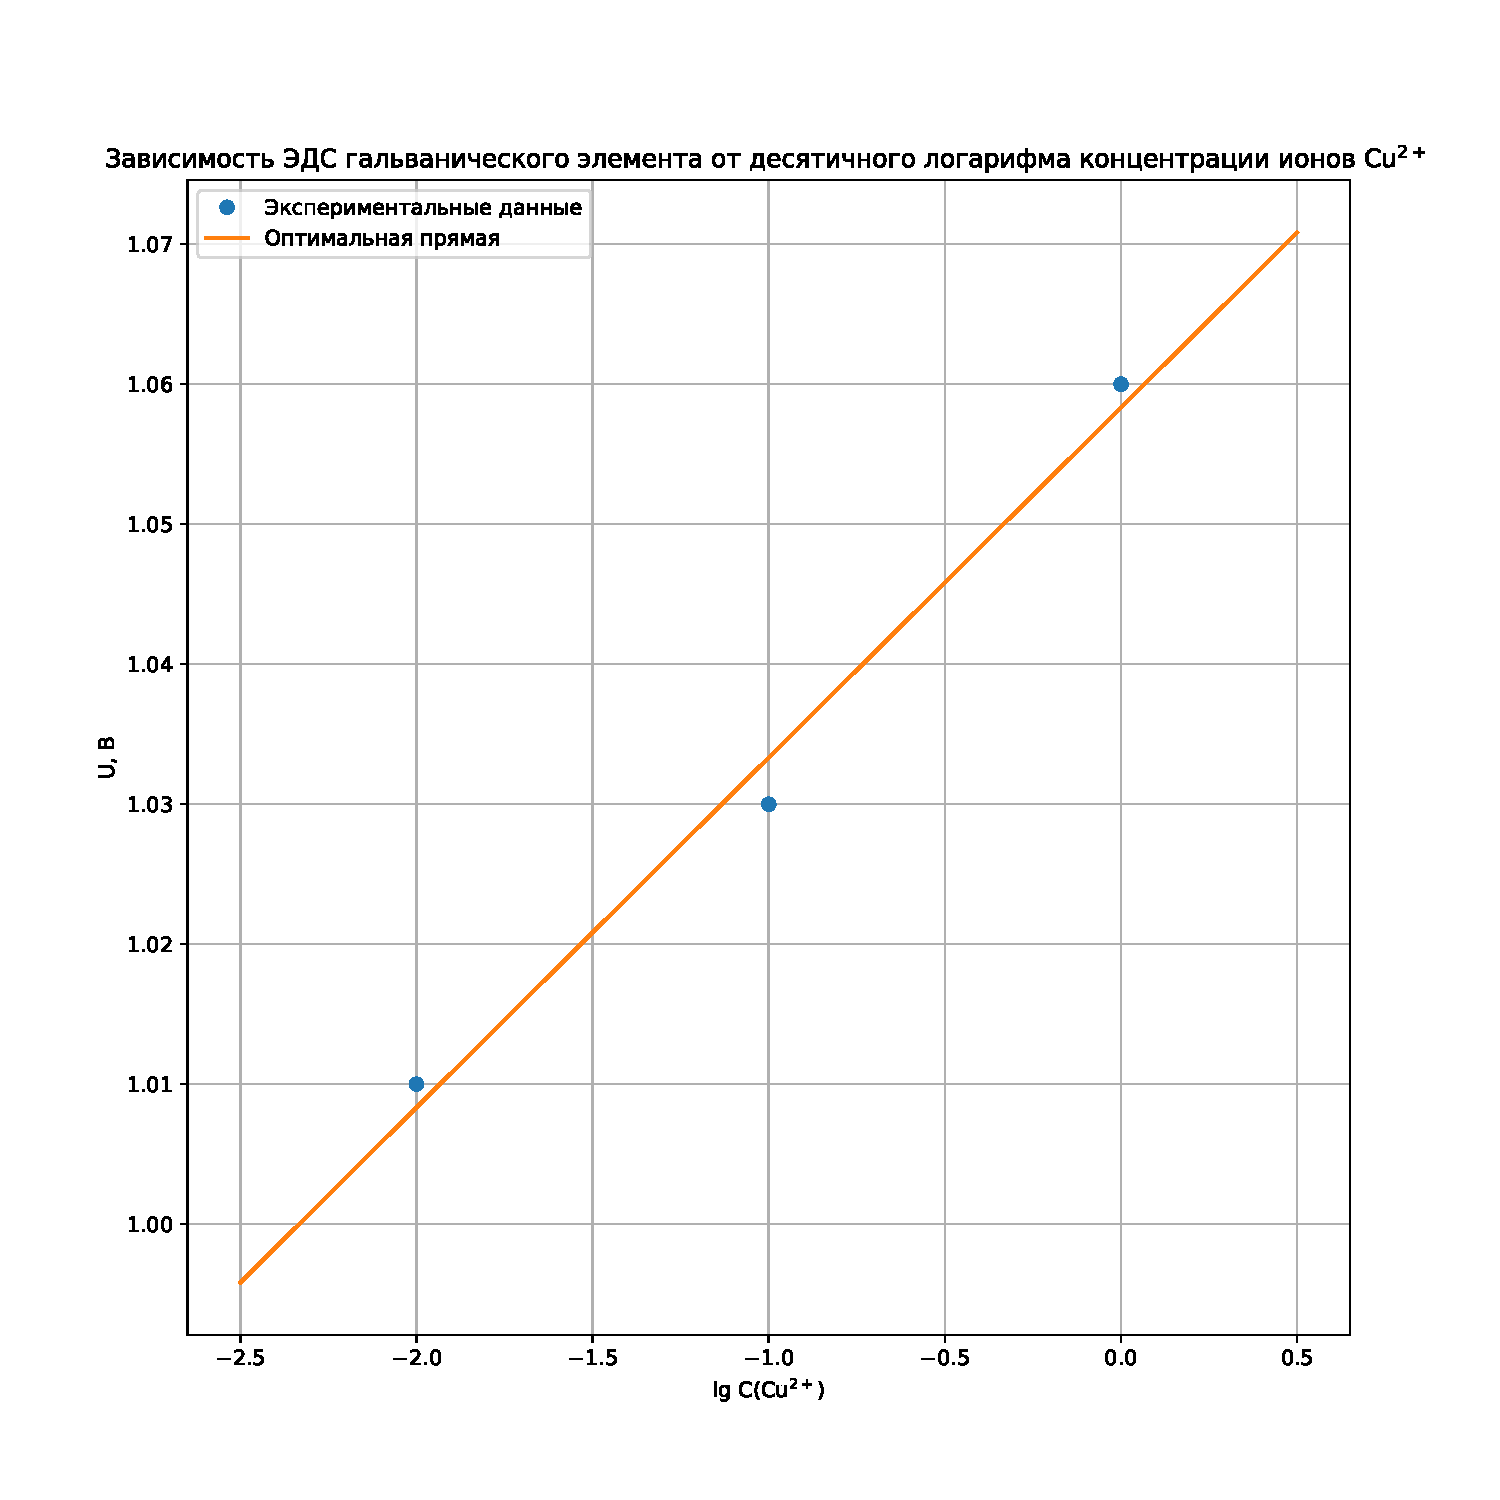
\includegraphics[width=0.7\linewidth]{eds}
\end{figure}

Коэффициент наклона прямой оказывается равным 0.026, что неплохо стыкуется с теоретическим ($0.059 / 2 = 0.0295$).

\subsection{Опыт 2: Электролиз растворов электролитов}

\subsubsection{Реактивы и оборудование}

\begin{itemize}
	\item Растворы: \ce{NaCl} (1M), \ce{KI}, \ce{K3[Fe(CN)6]}, фенолфталеина
	
	\item Инертные электроды (2 шт)
	\item Железный электрод
	\item Электролизеры (2 шт)
	\item Источник питания
	\item Фильтровальная бумага
	\item Шпатель для реактивов
	\item Стеклянная палочка
	\item Штатив
\end{itemize}

\subsubsection{Порядок выполнения опыта}

\subsubsection*{а)}

Электролизер был заполнен раствором \ce{NaCl} (1M), после чего в него были погружены два инертных электрода. В раствор было также добавлено 3 капли фенолфталеина. Затем был включен источник питания (ток электролиза $\approx 90$~mА)

На катоде при этом: \ce{Na+ + e -> Na^0}. Полученный натрий реагирует с водой с выделением водорода, который мы и видим (пузырьки газа):

\begin{equation}
	\ce{2Na + 2H2O -> 2NaOH + H2}
\end{equation}

На аноде же: \ce{2Cl- - 2e -> Cl2^0}. Получаемый хлор окрашивает фильтровальную бумажку, пропитанную раствором \ce{KI}, в фиолетовый цвет \ce{I2}:

\begin{equation}
	\ce{2KI + Cl2 -> 2KCl + I2}
\end{equation}

С помощью фенолфталеина около катода отслеживается щелочная среда.

\subsubsection*{б)}

Был проведен аналогичный эксперимент, только теперь инертный электрод на положительном полюсе был заменен железным. В результате на катоде реакция на катоде не поменялась, а вот на аноде хлор начал реагировать с железом электрода:

\begin{equation}
	\ce{Cl2 + Fe -> FeCl2}
\end{equation}

Это подтверждается реакцией с красной кровяной солью, которая была добавлена в раствор (качественная реакция на ионы \ce{Fe^2+}):

\begin{equation}
	\ce{Fe^{2+} + 3[Fe(CN)6] -> Fe4[Fe(CN)6]3}
\end{equation}

Осадок имеет вид темно-синих кристаллов.


\newpage

\fancyhead[R]{\textsc{Химические свойства галогенов и их соединений}}%Вставить колонтитул сюда

\section{Химические свойства галогенов и их соединений}

% Норм реакция

\subsection{Опыт 1: Получение бромной воды и йодной воды}

\subsubsection{Реактивы и оборудование}

\begin{itemize}
	\item Сухие соли: \ce{KBr}, \ce{KI}
	\item Растворы: \ce{HCl} (1M), \ce{NaClO}
	
	\item Пробирки
	
	\item Стеклянная палочка
	
	\item Шпатель для реактивов
\end{itemize}

\subsubsection{Порядок выполнения опыта}

В пробирку были помещены 2-3 микрошпателя \ce{KBr}, к которому был прибавлен 1 мл \ce{HCl} (1M), после чего содержимое пробирки было перемешано до растворения. Затем осторожно, по каплям, в пробирку был добавлен раствор \ce{NaClO}. В результате этого раствор поменял цвет с бесцветного на желтоватый.

Аналогичные действия были проведены с \ce{KI}, но раствор поменял цвет на коричневый.

\begin{align}
	\ce{HCl + KBr &-> KCl + HBr}\\
	\ce{HCl + KI &-> KCl + HI}
\end{align}

\begin{align}
	\ce{NaClO + 2HBr -> Br2 + NaCl + H2O}\\
	\ce{NaClO + 2HI -> NaCl + I2 + H2O}
\end{align}

%Норм реакция, гексан фиолетовый, т.е. йод

\subsection{Опыт 2: Сравнение окислительных свойств галогенов}

\subsubsection{Реактивы и оборудование}

\begin{itemize}
	\item Растворы: \ce{KI}, \ce{Br2}-вода
	
	\item Гексан
	
	\item Пробирки
	
	\item Стеклянная палочка
	
	\item Стакан
\end{itemize}

\subsubsection{Порядок выполнения опыта}

В пробирку был налит 1 мл раствора \ce{KI}, который был залит 1 мл гексана. К полученной жидкости был прилит 1 мл бромной воды, после чего раствор был перемешан. В результате этого гексан окрасился в фиолетовый цвет, что означает ожидаемое из уравнения реакции присутствие в нем \ce{I2}.

\begin{align}
	\ce{2KI + Br2 -> 2KBr + I2}
\end{align}

% Непонятно че с реакциями и зачем гексан в них

\subsection{Опыт 3: Восстановительная активность галогенид-ионов}

\subsubsection{Реактивы и оборудование}

\begin{itemize}
	\item Сухие соли: \ce{KBr}, \ce{KI}, \ce{H2SO4\text{(конц.)}}
	
	\item Гексан
	
	\item Пробирки
	
	\item Шпатель
	
	\item Стеклянная палочка
	
	\item Стакан
	
	\item Пипетка
\end{itemize}

\subsubsection{Порядок выполнения опыта}

В одну пробирку было помещено несколько кристаллов \ce{KBr}, в другую --- \ce{KI}. После этого в каждую из них было добавлено 2-3 капли концентрированной \ce{H2SO4}. При этом началась бурная реакция с выделением газа, имеющего запах зажженной спички (для \ce{KBr}) и сероводорода (для \ce{KI}). После этого был прилит небольшой объем воды и наслоен органический растворитель. Цвет содержимого пробирок оказался бледно-желтым (для \ce{KBr}) и фиолетовым для \ce{KI}.

\begin{align}
	\ce{2H2SO4 + 2 KBr -> SO2 + Br2 + K2SO4 + 2H2O}\\
	\ce{9H2SO4 + 8 KI -> 8KHSO4 + 4 I2 + H2S + 4H2O}
\end{align}

% Норм реакции

\subsection{Опыт 4: Качественные реакции на галогенид-ионы}

\subsubsection{Реактивы и оборудование}

\begin{itemize}
	\item Растворы: \ce{NaCl}, \ce{KBr}, \ce{KI}, \ce{Pb(NO3)2}
	
	\item Пробирки
\end{itemize}

\subsubsection{Порядок выполнения опыта}

В три пробирки были помещены 3-5 капель растворов солей: \ce{NaCl}, \ce{KBr}, \ce{KI}. В каждую из пробирок был прилит раствор \ce{Pb(NO3)2}. В результате в пробирках выпали осадки: белый мутный в пробирке с \ce{NaCl}, ярко-желтый в пробирке с \ce{KBr} и белый (полупрозрачный) в пробирке с \ce{KI}. Можно сделать вывод о применимости \ce{Pb(NO3)2} для нахождения йодид-ионов, однако необходима дополнительная реакция как минимум для установления их отличия от бромидов. %Какой вывод-то??

\begin{align}
	\ce{2NaCl + Pb(NO3)2 &-> PbCl2 + 2 NaNO3}\\
	\ce{2KBr + Pb(NO3)2 &-> PbBr2 + 2 KNO3}\\
	\ce{2KI + Pb(NO3)2 &-> PbI2 + 2 KNO3}\\
\end{align}

% Норм реакции

\subsection{Опыт 5: Взаимодействие брома и йода со щелочами}

\subsubsection{Реактивы и оборудование}

\begin{itemize}
	\item \ce{Br2}-вода, \ce{I2}-вода
	
	\item Растворы: \ce{NaOH}, \ce{H2SO4} (1M)
	
	\item Индикаторная бумага
	
	\item Пробирки
	
	\item Пипетка
\end{itemize}

\subsubsection{Порядок выполнения опыта}

К 5-6 каплям бромной воды был добавлен по каплям раствор \ce{NaOH} (1M) до обесцвечивания раствора. После этого раствор был подкислен несколькими каплями \ce{H2SO4} (1M), в ходе чего раствор вернул свой первоначальный цвет. Аналогичное наблюдалось при замене бромной воды йодной.

Цвет меняется из-за постепенного перехода \ce{Br2} (\ce{I2}) в бесцветные \ce{NaBr} и \ce{NaBrO} (\ce{NaI} и \ce{NaIO3}) в щелочной среде и обратно в кислотной.

\begin{align}
	\ce{Br2 + 2NaOH &-> NaBr + NaBrO + H2O}\\
	\ce{3I2 + 6NaOH &-> 5NaI + NaIO3 + 3H2O}
\end{align}

\begin{align}
	\ce{NaBr + NaBrO + H2SO4 &-> Na2SO4 + H2O + Br2}\\
	\ce{5NaI + NaIO3 + 3H2SO4 &-> 3Na2SO4 + 3H2O + 3I2}
\end{align}

\newpage

\fancyhead[R]{\textsc{Свойства неметаллов IV-VI групп и их соединений}}

\section{Свойства неметаллов IV-VI групп и их соединений}

\subsection{Опыт 1: Осаждение сульфидов и их свойства}

\subsubsection{Реактивы и оборудование}

\begin{itemize}
	\item Растворы: \ce{ZnCl2}, \ce{CuSO4}, \ce{FeCl2}, \ce{FeCl3}, \ce{MnCl2}, \ce{Na2S}, \ce{HCl}
	
	\item Пробирки
\end{itemize}

\subsubsection{Порядок выполнения опыта}

В 4 пробирки были налиты по 1 мл растворов \ce{ZnCl2}, \ce{CuSO4}, \ce{FeCl3}, \ce{MnCl2}, после чего в каждую из пробирок было добавлено по несколько капель раствора \ce{Na2S}. В результате в пробирках были получены осадки следующих цветов (в том же порядке, в котором указаны соли): молочно-белого, черного, черного и персикового. После этого в каждую из пробирок был добавлен раствор \ce{HCl} в результате чего с осадками произошло следующее  (в том же порядке, в котором указаны соли): осадок растворился (раствор стал голубовато-лунным), раствор позеленел, раствор посерел, раствор стал прозрачным.
\begin{align}
	\ce{ZnCl2 + Na2S &-> ZnS + 2 NaCl}\\
	\ce{CuSO4 + Na2S &-> CuS + Na2SO4}\\
	\ce{2FeCl3 + 3Na2S &-> 2 FeS + S + 6 NaCl}\\
	\ce{MnCl2 + Na2S &->  MnS + NaCl}
\end{align}

\begin{align}
	\ce{ZnS + 2HCl &-> H2S + ZnCl2}\\
	\ce{CuS + 2HCl &-> H2S + CuCl2}\\
	\ce{FeS + 2HCl &-> H2S + FeCl2}\\
	\ce{MnS + 2HCl &-> H2S + MnCl2}
\end{align}

\subsection{Опыт 2: Восстановительные свойства сульфидов}

\subsubsection{Реактивы и оборудование}

\begin{itemize}
	\item Раствор \ce{Na2S}
	
	\item \ce{Br2}-вода, \ce{I2}-вода
	
	\item Пробирки
\end{itemize}

\subsubsection{Порядок выполнения опыта}

В две пробирки было налито по 1 мл раствора \ce{Na2S}, после чего в одну пробирку был добавлен 1 мл бромной воды, в другую --- йодной. В результате в обеих пробирках выпал желтовато-белый осадок.

\begin{align}
	\ce{Na2S + Br2 &-> S + 2NaBr}\\
	\ce{Na2S + I2 &-> S + 2NaI}
\end{align}

\subsection{Опыт 3: Получение серы и растворение ее в щелочи}

\subsubsection{Реактивы и оборудование}

\begin{itemize}
	\item Растворы: \ce{Na2S2O3}, \ce{H2SO4}, \ce{NaOH}
	
	\item Пробирки
	
	\item Стеклянная палочка
	
	\item Спиртовка
\end{itemize}

\subsubsection{Порядок выполнения опыта}

В пробирку был налит 1 мл раствора \ce{Na2S2O3}, к которому было прибавлено несколько капель разбавленной \ce{H2SO4}. Спустя некоторое время в пробирке выпал желтовато-белый осадок. Затем в пробирку постепенно, по каплям, добавлялся раствор \ce{NaOH} до полного растворения осадка. % растворилась сера, белый Na2SO4 никуда не делся блен...

\begin{align}
	\ce{Na2S2O3 + H2SO4 &-> S + Na2SO4 + H2SO4}\\
	\ce{3S + 6NaOH &-> 3 H2O + Na2SO3 + 2 Na2S}
\end{align}

\subsection{Опыт 4: Свойства солей аммония}

\subsubsection{Реактивы и оборудование}

\begin{itemize}
	\item Сухие соли: \ce{(NH4)2CO3}, \ce{NH4Cl}
	
	\item Пробирки
	
	\item Спиртовка
\end{itemize}

\subsubsection{Порядок выполнения опыта}

В сухую пробирку было помещено немного \ce{(NH4)2CO3}, после чего пробирка была нагрета. В результате появился сильный запах аммиака. Аналогичный опыт был проведен с \ce{NH4Cl}: в этом случае также был запах аммиака (однако более слабый), а на стенках пробирки появился белый налет. Объясняется он тем, что получившиеся в ходе реакции газы вновь объединяются на более холодных стенках пробирки.

\begin{align}
	\ce{(NH4)2CO3 &-> H2O + CO2 + 2 NH3}\\
	\ce{NH4Cl &-> HCl + NH3}
\end{align}

% Реакция с растворением в воде похожа на говно

\subsection{Опыт 5: Разложение нитрата калия}

\subsubsection{Реактивы и оборудование}

\begin{itemize}
	\item Сухая соль \ce{KNO3}
	
	\item Растворы: \ce{H2SO4}, \ce{KMnO4}
	
	\item Пробирки
	
	\item Шпатель
	
	\item Лучина
	
	\item Спиртовка
\end{itemize}

\subsubsection{Порядок выполнения опыта}

В сухую пробирку было внесено 1-2 микрошпателя \ce{KNO3}, после чего пробирка была нагрета на пламени спиртовки до расплавления соли и дальнейшего его кипения. После этого в пробирку была внесена тлеющая лучина, которая при внесении чуть-чуть загорелась, что свидетельствует о наличии в пробирке кислорода. Полученный осадок был растворе в 1 мл дистиллированной воды с добавлением большого объема \ce{H2SO4} (1M) и раствора \ce{KMnO4}, в результате чего раствор расслоился: снизу он был бесцветным, сверху --- фиолетово-розовым. Сверху, по всей видимости, оказался \ce{MnSO4}, снизу --- соли калия. % Проверить вывод.

\begin{align}
	\ce{KNO3 &-> KNO2 + O2}\\
	\ce{5 KNO2 + 3 H2SO4 + 2 KMnO4 &-> 3 H2O + K2SO4 + 5 KNO3 + 2 MnSO4}
\end{align}

\subsection{Опыт 6: Качественная реакция на анионы}

\subsection*{а) Качественное обнаружение соединений серы}
\subsubsection{Реактивы и оборудование}

\begin{itemize}
	\item Растворы: \ce{Na2S}, \ce{HCl} (1M), \ce{PbSO4}, \ce{BaCl2}, \ce{Na2SO3}, \ce{KMnO4}, \ce{KI}, \ce{Na2S2O3}, \ce{FeCl3}
	
	\item Пробирки
	
	\item Фильтровальная бумага
\end{itemize}

\subsubsection{Порядок выполнения опыта}

\begin{itemize}
\item 

В пробирку был внесен раствор \ce{Na2S}, который был смешан с \ce{HCl} (1M). Пробирка была накрыта фильтровальной бумажкой, смоченной раствором \ce{Pb(NO3)2}. Бумажка окрасилась в черный цвет \ce{PbS}.

\begin{align}
	\ce{Na2S + 2HCl &-> 2 NaCl + H2S}\\
	\ce{H2S + Pb(NO3)2 &-> 2 HNO3 + PbS}
\end{align}

\item

В пробирку было внесено несколько капель \ce{Na2SO4}, после чего раствор был подкислен парой капель \ce{HCl} (1M). Затем в пробирку было прибавлено несколько капель \ce{BaCl2}, в результате чего выпал белый мутный осадок.

\begin{equation}
	\ce{Na2SO4 + BaCl2 -> 2 NaCl + BaSO4}
\end{equation}

\item 

В две пробирки было налито по 1 мл раствора \ce{Na2SO3}, который был подкислен парой капель \ce{HCl} (1M). В первую пробирку было добавлено 3 капли раствора \ce{KMnO4}, который в ходе реакции обесцветился. Затем в пробирку был внесен \ce{BaCl2}, вследствие чего в пробирке выпал белый осадок. Во вторую же пробирку было добавлено 3 капли \ce{KI}, в результате чего раствор получил лимонно-зеленую окраску. % Проверь окраску потом, дальтоник

% Нет реакции с хлоридом бария

\begin{align}
	\ce{2 KMnO4 + 6 HCl + 5 Na2SO3 -> 5 Na2SO4 + 2MnCl2 + 2KCl + 3H2O}\\
	\ce{Na2SO3 + 6 KI + 6 HCl -> 3 I2 + 6 KCl + 3H2O + Na2S}
\end{align}

\item 

В пробирку был внесен раствор \ce{Na2S2O3}, к которому был добавлен раствор \ce{FeCl3}. В результате окраска раствора стала коричневой (была оранжево-ржавой).

\begin{equation}
	\ce{2 Na2S2O3 + 2FeCl -> 2 FeCl2 + Na2S4O6 + 2 NaCl}
\end{equation}
\end{itemize}

\subsection*{б) Качественное обнаружение соединений азота}

\subsubsection{Реактивы и оборудование}

\begin{itemize}
	\item Растворы: \ce{KNO3}, \ce{NaOH} (1M), \ce{NaNO2}, \ce{HCl} (1M), \ce{KMnO4}, \ce{KI}, \ce{BaCl2}, \ce{NH4Cl}
	
	\item \ce{Zn} порошок
	
	\item Пробирки
	
	\item Шпатель
	
	\item Спиртовка
	
	\item Индикаторная бумага
	
	\item Фильтровальная бумага
\end{itemize}

\subsubsection{Порядок выполнения опыта}

\begin{itemize}
\item

В пробирку был внесен небольшой объем \ce{KNO3} вместе с 2 микрошпателями порошка \ce{Zn} и 1 мл раствора \ce{NaOH} (1M), после чего пробирка и ее содержимое были нагреты. В результате из пробирки начал выделяться запах аммиака. При внесении в выделяющийся газ универсальной индикаторной бумаги, смоченной воды, она показала щелочную среду, что косвенно свидетельствует о том, что газ --- \ce{NH3}.

\begin{equation}
	\ce{8 Zn + 14 NaOH + 2 KNO3 -> K2ZnO2 + 7Na2ZnO2 + 2NH3 + 4H2O}
\end{equation}

\item % Надо написать

В две пробирки был внесен \ce{NaNo2}, после чего в одну из пробирок был прилит раствор \ce{KMnO4}, в результате чего раствор \ce{KMnO4} потерял окраску. В другую же пробирку было добавлено 3 капли \ce{KI}, после чего раствор стал фиолетовым (?). Затем в обе пробирки был добавлен раствор \ce{BaCl2}, вследствие чего .

% Нет реакций с BaCl2

\begin{align}
	\ce{5NaNO2 + 2KMnO4 + 6HCl -> 5 NaNO3 + 2 MnCl2 + 2 KCl + 3H2O}\\
	\ce{2 NaNO2 + 2 KI + 4 HCl -> I2 + 2 KCl + 2NO + 2 NaCL + 2H2O}
\end{align}

\item 

% Тут вообще мутная тема со всем этим лакмусом, нужно аккуратно будет все это сверить.

В проибрку был внесен 1 мл раствора \ce{NH4Cl} и добавлены 3 капли раствора \ce{NaOH} (1M). После этого пробирка была нагрета, вследствие чего из нее начал выделяться запах аммиака. При внесении в выделяющийся газ универсальной индикаторной бумаги, смоченной воды, она показала щелочную среду, что косвенно свидетельствует о том, что газ --- \ce{NH3}.

\begin{equation}
	\ce{NH4Cl + NaOH -> NH3 + H2O + NaCl}
\end{equation}
\end{itemize}

\end{document}